\documentclass[a4paper,12pt]{article}
\usepackage[utf8]{inputenc}
\usepackage[english]{babel}
\usepackage{authblk}
\usepackage{graphicx}
\usepackage{mathptmx}
\usepackage[singlespacing]{setspace}
\usepackage[headheight=1in,margin=1in]{geometry}
\usepackage{fancyhdr}
\usepackage{lipsum}


\renewcommand{\headrulewidth}{0pt}
\pagestyle{fancy}


\makeatletter
\def\@maketitle{%
  \newpage

  \begin{center}%
  \let \footnote \thanks
    {\LARGE \@title \par}%
  \end{center}%
  \par
  \vskip 0.1em}
\makeatother

\chead{%
  $11$$^{th}$ International Conference on Computational Social Science IC$^{2}$S$^{2}$\\
  July 21-24, 2025, Norrköping, Sweden%
}

\graphicspath{{images/}}

\title{Developing a Large Language Model System for Swiss Cases on Choice of Law}

 
\date{}

\begin{document}

\maketitle
\thispagestyle{fancy}

\begin{center}
\textit{Keywords: NLP, LLMs, LLM Evaluation, Court Decisions, Private International Law}
\newline
\end{center}

\section*{Extended Abstract}

Introduction

Based on a data sample of 33 cases on choice of law, this study describes the development of a customized Large Language Model (LLM) system for private international law. The LLM system is equipped to handle three languages (German, French, and Italian) and handles expert input in English. This mirrors - on a small scale - the multilingual challenges encountered in our field.

The goal of this machine-learning experiment is to obtain high-quality legal analyses from the LLM system in four key categories: Relevant facts, choice of law issue, relevant rules of law, and court's position. The research endeavor is centered around determining if it is possible for LLMs to produce analyses comparable to those of legal professionals. Furthermore, it will be assessed to what extent an automated evaluation can contribute to determining the quality of the LLM-generated outputs.

OpenAI's XXX model, a pre-trained language model, is the primary model employed in this experiment. It uses advanced vectorization and embedding techniques. However, can this numerical representation capture the nuanced reasoning of case law interpretation?

- explain Court Decision Analysis for CoL

	- explain JD differences and why they matter

  - explain original procedure with human evaluation

In a first installment of the experiment, the automated answers were generated and then given to a human legal expert for evaluating each court decision and each answering category with a previously defined set of evaluation metrics. The legal expert also made notes on specific intricacies they could identify from reading the automatically generated answers. This (timely!) effort allows for a particularly nuanced insight into the performance of the LLM. On a larger scale it quickly becomes inefficient/expensive to have every answer generated by an LLM reviewed by a human.

- explain goal of comparing evaluation methods

Thus, an automated evaluation approach might prove useful. To figure out the trustworthiness of such automated approaches, the following metrics are computed and compared:

GEval vs Human Evaluation

GEval vs GEval with reference text

GEval vs BERTScore

- explain goal of comparing different LLMs

\section*{References}
...

\vskip 40pt
\underline {Guidelines:}
\begin{itemize}
\itemsep0pt
  \item 2 pages maximum (excluding references, figures and tables)
  \item Single spaced
  \item Font size 12pt
  \item 1-inch margins
  \item Do not include author names for blind review and remove any information that may identify the author(s)
\end{itemize}

\underline {Include in Order:}
\begin{itemize}
\itemsep0pt
  \item Paper title
  \item 5 keywords
  \item Extended abstract 
  \item References
  \item Figure or Table
\end{itemize}

\newpage

\begin{figure}[htp]
\centering
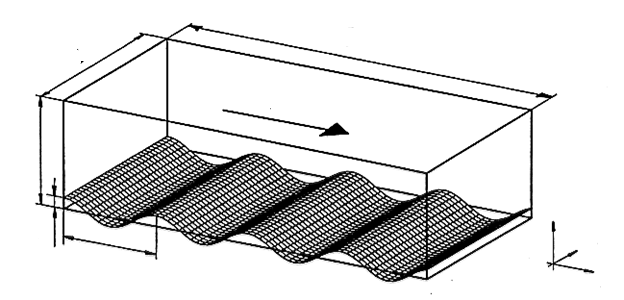
\includegraphics[width=14cm]{figexample.png}
\caption{Ut sed risus ut ante consectetur ultricies}
\label{fig:image}
\end{figure}

\end{document}
